\documentclass[tikz,border=8pt]{standalone}
% Shared look for every TikZ diagram. Load with \input{../../tools/tikz-style.tex}
\usepackage[T1]{fontenc}
\usepackage{lmodern}
\renewcommand{\sfdefault}{lmr}  % diagrams use the same serif as the text
\usetikzlibrary{arrows.meta, positioning, shapes.geometric, calc, fit, backgrounds}
\definecolor{cblue}{HTML}{4C78A8}
\definecolor{corange}{HTML}{F58518}
\definecolor{cgreen}{HTML}{54A24B}
\definecolor{cred}{HTML}{E45756}
\definecolor{cpurple}{HTML}{B279A2}
\definecolor{cgrey}{HTML}{6B6B6B}
\tikzset{
  every picture/.style={font=\sffamily, line width=1.2pt},
  box/.style={draw=#1, fill=#1!12, rounded corners=4pt, align=center, inner sep=7pt, minimum height=1.1cm},
  box/.default=cgrey,
  arrow/.style={-{Stealth[length=3mm]}, draw=cgrey, line width=1.4pt},
  title/.style={font=\sffamily\bfseries\Large},
  note/.style={font=\sffamily\small, text=cgrey, align=center},
}
\AtBeginDocument{\hyphenpenalty=10000 \exhyphenpenalty=10000}

\begin{document}
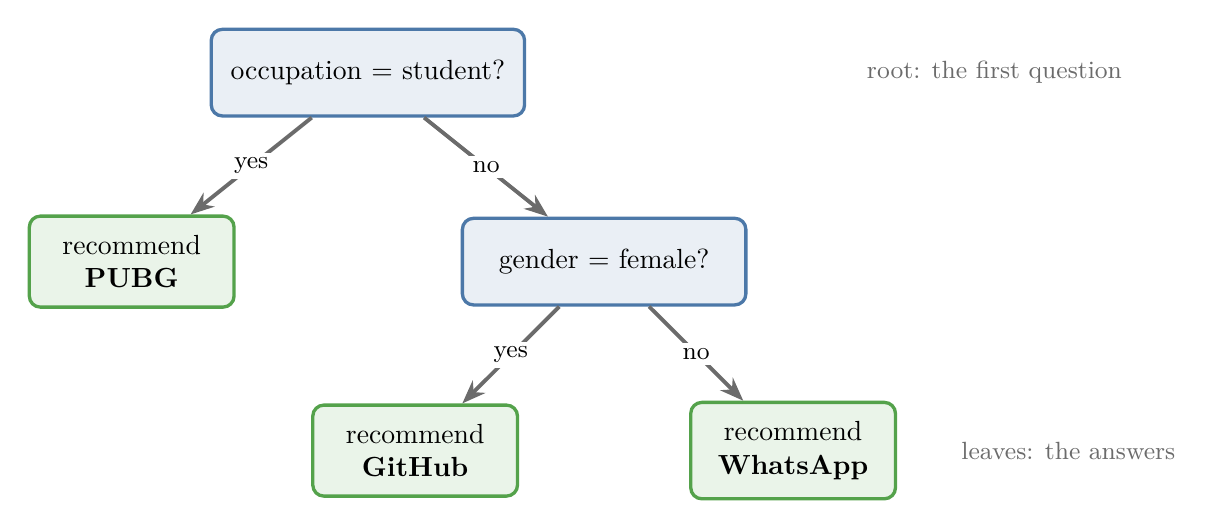
\begin{tikzpicture}[
  q/.style={box=cblue, minimum width=3.6cm},
  leaf/.style={box=cgreen, minimum width=2.6cm},
  lab/.style={font=\sffamily\small, fill=white, inner sep=2pt}]
  \node[q] (root) at (0,0) {occupation = student?};
  \node[leaf] (pubg) at (-3,-2.4) {recommend\\\textbf{PUBG}};
  \node[q] (g) at (3,-2.4) {gender = female?};
  \node[leaf] (gh) at (0.6,-4.8) {recommend\\\textbf{GitHub}};
  \node[leaf] (wa) at (5.4,-4.8) {recommend\\\textbf{WhatsApp}};
  \draw[arrow] (root) -- node[lab] {yes} (pubg);
  \draw[arrow] (root) -- node[lab] {no} (g);
  \draw[arrow] (g) -- node[lab] {yes} (gh);
  \draw[arrow] (g) -- node[lab] {no} (wa);
  \node[note, anchor=west] at (6.2,0) {root: the first question};
  \node[note, anchor=west] at (7.4,-4.8) {leaves: the answers};
\end{tikzpicture}
\end{document}
